\section{Introduction}
\label{chap:intro}

The know-how of designing and making buildings has seen tumultuous scales of updates as seen from huts to skyscrapers. 
 Before the advent the electricity, the buildings were conceived as a mere brick and mortar rendition for habitable and workable spaces. 
 When electrical appliances started populating households, the notion of passive space turned into a controllable environment using sensors and actuators.
However, most of the existing buildings were already constructed before the apparition of internet and world wide web in 1990.
This means building architectures were not developed keeping in mind the quantity, type and location of sensors.
The popularity of Internet of Thing (IoT) devices have lead to an ad-hoc assimilation in buildings that are usually situated in an environment of dynamic parameters like temperature, CO2, wind, etc.
Such an approach can lead to naive zonal distribution of sensors due to obscurity on spatio-temporal importance. 
Secondly, a streaming IoT sensor can act as a data source of sensitive patterns raising privacy concerns among stakeholders.
Thirdly, the cost of equipping spaces with embedded hardware over a large commercial space is non-negligible and comes with a recurring payment of powering up the solution.
In this work, we investigate if there is a way to determine a minimalist sensing solution for non-intrusive spatio-temporal coverage to lower the capital cost and energy footprint for a smart building solution. 


\noindent \textbf{Problem Setting.}
Let there be $Z$ locations in a building that are equipped with no more than $K$ types of sensors. 
We seek to find the optimal bipartite set of sensors coupled with a knowledge base to predict any one of the two sets using the other.
Let $\mathcal{H}^g$ represent the collective knowledge of a group $g$ that can contain multiple ambient sensors and power meters.
$\mathcal{H} = \{\mathcal{H}^g | \forall g \in G \}$ is built in a way to provide a predictive coverage over all $Z$ zones with $G$ logical partitions of sensors.
Then $Z \cap \mathcal{H}$ shall be semantically interpreted as the subset of spaces that are equipped with sensors.
So $\mathcal{H} - (Z \cap \mathcal{H})$ denotes the approximated knowledge of $Z \cap \mathcal{H}$ sensor-less zones.\\

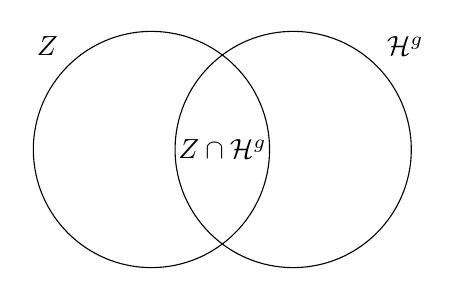
\begin{tikzpicture}
 \label{pic:sensorspacevenn}
% Set A
\node [draw,
    circle,
    minimum size =3cm,
    label={135:$Z$}] (A) at (0,0){};
 
% Set B
\node [draw,
    circle,
    minimum size =3cm,
    label={45:$\mathcal{H}^g$}] (B) at (1.8,0){};

 %\draw [red,dashed] (-0.5,0.5) rectangle (-10.5,10.5) node [black,below] {$K_S$};
% Set intersection label
%\node at (-0.6,0) {$Z - K_o$};
\node at (0.9,0) {$Z \cap \mathcal{H}^g$};
%\node at (2.1,0) {$K - Z_o$};
 
\end{tikzpicture}

The problem is to find the minimal working subset of sensors ($Z \cup \mathcal{H}$) to yield the best hypothesis space $\mathcal{H}^*$ with least prediction error.
The set $\mathcal{H}^*$ is termed as \textbf{virtual sensor field} because of its capability to replace an embedded hardware with a software approximation of the same.
 
In the upcoming sections we explain the context and motivation for the problem and formulate a distributed scalable solution.
Then, we study experimentally the effect of distinct semantic groupings on the virtualization accuracy, followed by a multi-objective optimization to discover the minimal sensor group. 
Finally we compare our results with a state of art work in optimal sensor placement to highlight key differences between the two types of problem. 
% Our work treats the sensor distribution across a building as a network of groups, where each group tries to optimizes the functional representation of the virtual sensor field.
% In doing so, the system utilises the collective knowledge to find a set of Pareto optimal solutions for placing sensors on the floor-plan.
% The motivation to reduce sensors adds a layer of controllable privacy for the occupants and minimizes the power required by hardware to run a smart building solution.

